% ============================================================
%  compare_equipo_03.tex: deck de comparación de algoritmos.
%  Se compila con XeLaTeX desde 04_slides/compile_slides.R. Las figuras y
%  tablas no se copian aquí: se leen de 02_outputs/, donde las escribe
%  01_code/13_compare_algorithms.R, para que el PDF siempre muestre los
%  resultados de la última corrida.
% ============================================================
\documentclass[aspectratio=169, 10pt]{beamer}

% ---------- Tema ----------
\usetheme{metropolis}

% ---------- Idioma y codificación ----------
\usepackage[utf8]{inputenc}
\usepackage[spanish,provide=*]{babel}
\usepackage[T1]{fontenc}

% ---------- Fuente: Calibri (vía Carlito, su equivalente libre) ----------
\usepackage{ifxetex,ifluatex}
\newif\ifxetexorluatex
\ifxetex\xetexorluatextrue\fi
\ifluatex\xetexorluatextrue\fi
\ifxetexorluatex
  \usepackage{fontspec}
  % Se carga por nombre de archivo para que XeLaTeX la encuentre tanto en
  % las fuentes del sistema como en la distribución de LaTeX (TinyTeX).
  \setmainfont{Carlito}[Extension = .ttf, UprightFont = *-Regular,
    BoldFont = *-Bold, ItalicFont = *-Italic, BoldItalicFont = *-BoldItalic]
  \setsansfont{Carlito}[Extension = .ttf, UprightFont = *-Regular,
    BoldFont = *-Bold, ItalicFont = *-Italic, BoldItalicFont = *-BoldItalic]
\else
  \PackageWarningNoLine{plantilla}{Compila con XeLaTeX o LuaLaTeX para usar la fuente Calibri/Carlito}
\fi

% ---------- Matemáticas ----------
\usepackage{amsmath, amssymb}

% ---------- Gráficos, tablas y código ----------
\usepackage{graphicx}
\graphicspath{{../02_outputs/figures/}}
\usepackage{tikz}
\usetikzlibrary{positioning, arrows.meta, shapes.geometric}
\usepackage{booktabs}
\usepackage{array}
\usepackage{changepage}
\usepackage{listings}

% ---------- Paleta de acento ----------
\definecolor{accent}{HTML}{2E5EAA}
\setbeamercolor{palette primary}{bg=accent, fg=white}
\setbeamercolor{progress bar}{fg=accent, bg=accent!20}
\setbeamercolor{frametitle}{bg=accent}
\setbeamercolor{alerted text}{fg=accent}

% ---------- Ajustes de Metropolis ----------
\setbeamertemplate{section in toc}[sections numbered]
\setbeamertemplate{frame numbering}[fraction]
\metroset{block=fill, sectionpage=none, numbering=fraction, progressbar=none}

% ---------- Ajustes propios ----------
% Cajas (block) con margen interno, para que el texto no toque los bordes.
\setbeamertemplate{block begin}{%
  \par\vskip\medskipamount%
  \begin{beamercolorbox}[colsep*=.5ex, leftskip=0.4ex, sep=0.9ex, vmode]{block title}%
    \usebeamerfont*{block title}\insertblocktitle%
  \end{beamercolorbox}%
  \nointerlineskip%
  \begin{beamercolorbox}[colsep*=.5ex, leftskip=0.4ex, sep=1ex, vmode]{block body}%
    \usebeamerfont{block body}%
    \begin{adjustwidth}{0pt}{2.5ex}%
}
\setbeamertemplate{block end}{\end{adjustwidth}\end{beamercolorbox}\vskip\smallskipamount}
% Nota pequeña al pie de una diapositiva (fuente de los datos).
\newcommand{\nota}[1]{\vfill{\scriptsize\color{black!60}#1\par}}
% Las slides de respaldo no cuentan en la numeración.
\usepackage{appendixnumberbeamer}

% ============================================================
%  Datos de portada
% ============================================================
\title{Comparaci\'on de algoritmos}
\subtitle{¿Qu\'e algoritmo predice mejor la pobreza de los hogares?}
\author{Equipo 03: Juli\'an Herrera, Andr\'es Silva y Valentina Vera}
\institute{MECA 4107 Big Data y Machine Learning para Econom\'ia Aplicada, Universidad de los Andes}
\date{28 de octubre de 2026}

% ============================================================
\begin{document}

\maketitle

% ============================================================
\section{Mejor modelo}
% ============================================================

\begin{frame}{Mejor modelo: LightGBM con 1.296 variables, 0,77 en Kaggle}
  \begin{columns}[T, onlytextwidth]
    \begin{column}{0.44\textwidth}
      \begin{block}{Especificaci\'on}
        \footnotesize
        \begin{itemize}\setlength{\itemsep}{1pt}
          \item Boosting de gradiente (LightGBM)
          \item Conjunto X\_7: 1.296 variables del hogar y de sus miembros
          \item 31 hojas por \'arbol, tasa de aprendizaje 0,04, 748 rondas
          \item Penalidades L2 = 10 y L1 = 0,1
          \item Umbral 0,39, el que maximiza el F1 en validaci\'on cruzada
        \end{itemize}
      \end{block}
      \begin{center}
        {\LARGE\bfseries\color{accent}0,77}\\[0.5mm]
        {\small F1 en Kaggle (tabla p\'ublica)}\\[0.5mm]
        {\scriptsize F1 CV 0,768 \,·\, precisi\'on 0,744 \,·\, recall 0,794}
      \end{center}
    \end{column}
    \begin{column}{0.52\textwidth}
      \begin{block}{Lo que muestra la comparaci\'on}
        \small
        \begin{enumerate}
          \item \textbf{El algoritmo importa:} con las mismas 43 variables, el boosting obtiene el mayor F1 (0,731 frente a 0,715 de Random Forest y 0,711 de Elastic Net).
          \item \textbf{Gana porque ordena mejor a los hogares:} para encontrar a los mismos pobres, incluye unos 2.000 hogares no pobres menos que Elastic Net.
          \item \textbf{La informaci\'on importa m\'as:} describir mejor el hogar suma 3,7 puntos de F1; ajustar hiperpar\'ametros o rebalancear las clases, a lo sumo 1,1.
        \end{enumerate}
      \end{block}
    \end{column}
  \end{columns}
\end{frame}

% ============================================================
\section{Datos}
% ============================================================

\begin{frame}{Datos: predecir la pobreza sin observar el ingreso}
  \begin{columns}[c, onlytextwidth]
    \begin{column}{0.5\textwidth}
      \centering
      \small
      \begin{tabular}{lrr}
        \toprule
        & Train & Test \\
        \midrule
        Hogares & 164.960 & 66.168 \\
        Personas & 543.109 & 219.644 \\
        Variables de hogares & 23 & 16 \\
        Variables de personas & 135 & 63 \\
        Hogares pobres & 20,0\% & A predecir \\
        \bottomrule
      \end{tabular}

      \vspace{2mm}
      {\scriptsize Fuente: DANE, Misi\'on de Empalme (MESE). Hogares y personas se unen con el identificador del hogar.}
    \end{column}
    \begin{column}{0.46\textwidth}
      \footnotesize
      \begin{itemize}
        \item Un hogar es pobre si su ingreso per c\'apita est\'a por debajo de la l\'inea de pobreza.
        \item En test no est\'a el ingreso: faltan 7 variables de hogares y 72 de personas, casi todas montos de ingresos. Hay que predecir la pobreza con lo que se asocia al ingreso.
        \item Solo 1 de cada 5 hogares es pobre. Clasificar a todos como no pobres acierta el 80\%, pero no encuentra a ning\'un pobre: su F1 es 0.
        \item Por eso evaluamos con F1 y elegimos el umbral que lo maximiza.
      \end{itemize}
    \end{column}
  \end{columns}
\end{frame}

\begin{frame}{Predictores: de lo m\'as f\'acil de observar a lo m\'as detallado}
  \centering
  \vspace{3mm}
  {\footnotesize Como no vemos el ingreso, usamos variables que lo aproximan: cu\'antos generan ingreso, cu\'anto y con qu\'e calidad trabajan, entre cu\'antos se reparte y cu\'anto vale la vivienda.\par}
  \vspace{2mm}
  {\scriptsize 
\begin{tabular}{llrl}
\toprule
Conjunto & Contenido & Variables & Algoritmos evaluados\\
\midrule
X\_1 & Ubicación, tenencia de la vivienda, tamaño y hacinamiento & 5 & CART, Logit\\
X\_2 & + composición del hogar, dependencia y educación & 11 & CART, Logit\\
X\_3 & + ocupados e inactivos & 15 & CART, Logit\\
X\_4 & + horas, cotización, pensión y posición ocupacional & 21 & CART, Logit\\
X\_5 & + arriendo, desempleo, salud, subempleo y transferencias & 43 & Los 9 algoritmos\\
X\_6 & + miembros por categoría de educación, ocupación y empresa & 148 & LightGBM, XGBoost\\
X\_7 & Detalle del hogar y de cada miembro (con datos faltantes) & 1.296 & LightGBM, XGBoost\\
\bottomrule
\end{tabular}
}
  \nota{Cada conjunto contiene al anterior y agrega un bloque; X\_7 se construy\'o aparte y solo lo usan los algoritmos que manejan datos faltantes.}
\end{frame}

\begin{frame}{Datos: el efecto de un ocupado depende del tama\~no del hogar}
  \begin{columns}[c, onlytextwidth]
    \begin{column}{0.64\textwidth}
      \centering
      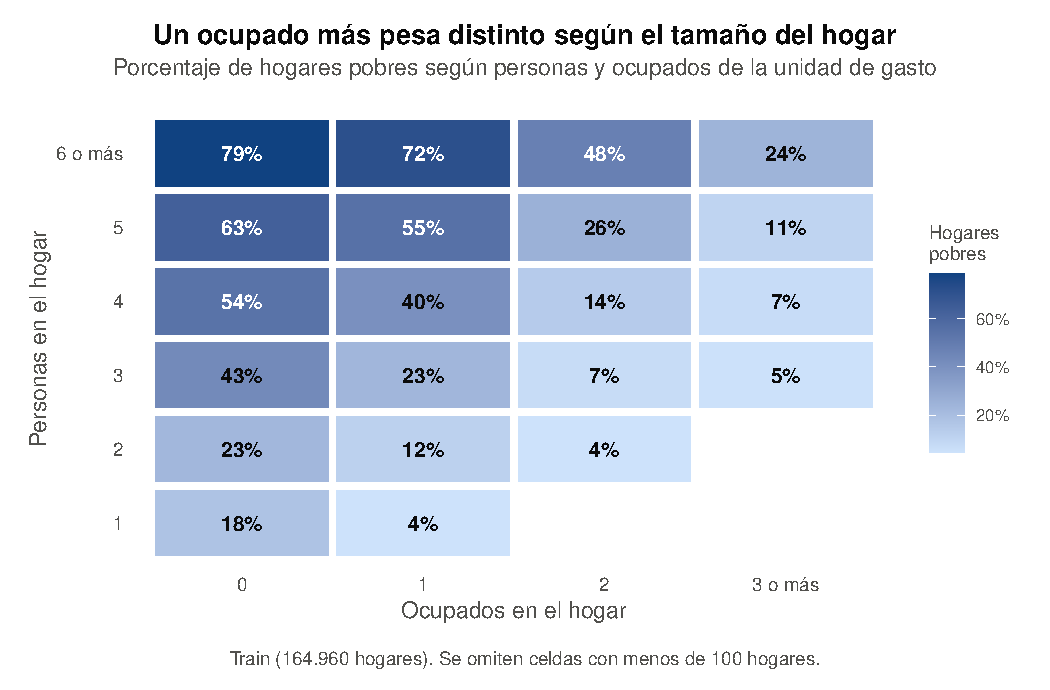
\includegraphics[width=\linewidth, height=0.82\textheight, keepaspectratio]{pobreza_ocupados_personas}
    \end{column}
    \begin{column}{0.33\textwidth}
      \footnotesize
      \begin{itemize}
        \item Ocupados y personas est\'an arriba y abajo en el ingreso per c\'apita: su efecto se combina.
        \item Pasar de 1 a 2 ocupados reduce la pobreza en 8 puntos en hogares de 2 personas y en 24 puntos en hogares de 6 o m\'as.
        \item Un modelo lineal suma el mismo efecto en todas las celdas; un \'arbol puede aprender que el efecto cambia.
      \end{itemize}
      \vspace{2mm}
      {\footnotesize\alert{\textbf{Hip\'otesis:} si el efecto de una variable depende de otra, a un modelo de \'arboles le deber\'ia ir mejor que a uno lineal.}}
    \end{column}
  \end{columns}
\end{frame}

\begin{frame}{Datos: el arriendo aproxima el ingreso, pero no en l\'inea recta}
  \begin{columns}[c, onlytextwidth]
    \begin{column}{0.64\textwidth}
      \centering
      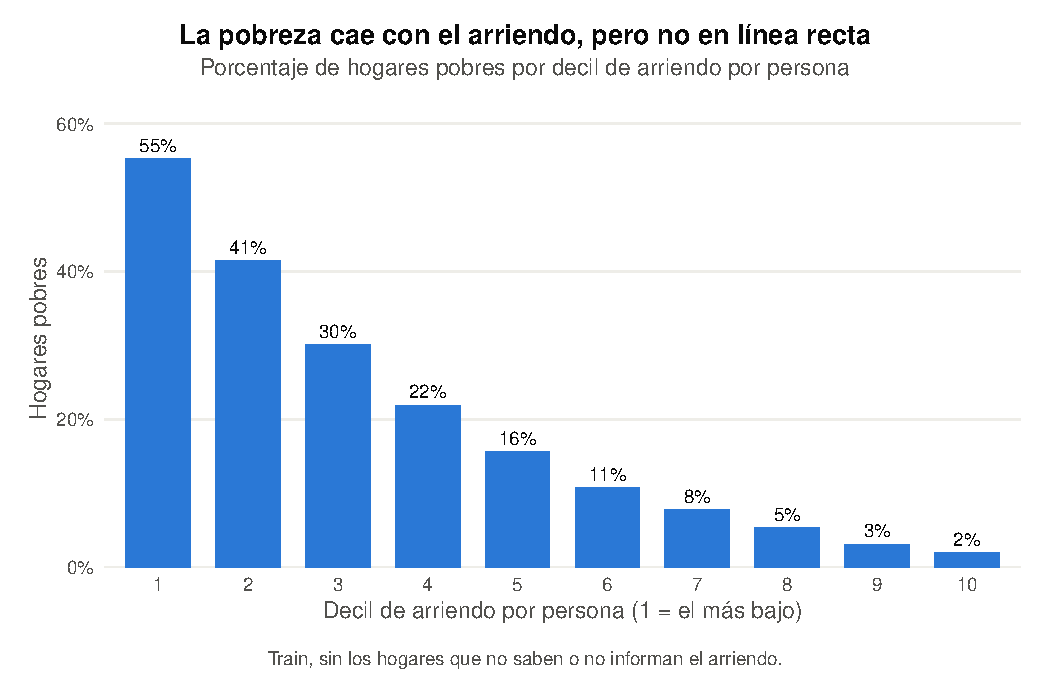
\includegraphics[width=\linewidth, height=0.82\textheight, keepaspectratio]{pobreza_arriendo_deciles}
    \end{column}
    \begin{column}{0.33\textwidth}
      \footnotesize
      \begin{itemize}
        \item El arriendo aproxima el valor de la vivienda, que refleja el ingreso.
        \item La pobreza cae del 55\% al 2\%, pero no pareja: 14 puntos del decil 1 al 2 y solo 1 del 9 al 10.
        \item Un modelo lineal necesita transformaciones hechas a mano; un \'arbol parte la variable donde cambia la pobreza.
      \end{itemize}
      \vspace{2mm}
      {\footnotesize\alert{\textbf{Hip\'otesis:} si el efecto cambia por tramos, a un modelo de \'arboles le deber\'ia ir mejor que a uno lineal.}}
    \end{column}
  \end{columns}
\end{frame}

% ============================================================
\section{Comparaci\'on de algoritmos}
% ============================================================

\begin{frame}{Probamos los siete algoritmos requeridos}
  \vspace{5mm}
  \centering
  {\small 
\begin{tabular}{lrrr}
\toprule
Algoritmo & Variantes evaluadas & Mejor F1 CV & Kaggle (misma variante)\\
\midrule
LPM & 2 & 0,688 & --\\
Logit & 5 & 0,711 & 0,71\\
Elastic Net & 1 & 0,711 & --\\
CART & 7 & 0,686 & 0,67\\
Random Forest & 3 & 0,715 & 0,71\\
Boosting & 8 & 0,768 & 0,77\\
Naive Bayes & 2 & 0,644 & 0,64\\
\bottomrule
\end{tabular}
}

  \vspace{4mm}
  \begin{columns}[T, onlytextwidth]
    \begin{column}{0.48\textwidth}
      \footnotesize
      \begin{itemize}
        \item 28 variantes, todas evaluadas con los mismos 5 folds de validaci\'on cruzada.
        \item El F1 de validaci\'on cruzada anticipa bien el de Kaggle: la diferencia es de 0,016 o menos.
      \end{itemize}
    \end{column}
    \begin{column}{0.48\textwidth}
      \footnotesize
      \begin{itemize}
        \item Boosting incluye XGBoost, LightGBM y AdaBoost.
        \item El mejor resultado de cada algoritmo usa conjuntos distintos: para comparar algoritmos hay que fijar las variables.
      \end{itemize}
    \end{column}
  \end{columns}
  \nota{--: esa variante no se envi\'o a Kaggle. LPM y Elastic Net s\'i se enviaron, con otras especificaciones (0,68 y 0,69).}
\end{frame}

\begin{frame}{En igualdad de condiciones: las mismas 43 variables}
  \begin{columns}[c, onlytextwidth]
    \begin{column}{0.66\textwidth}
      \centering
      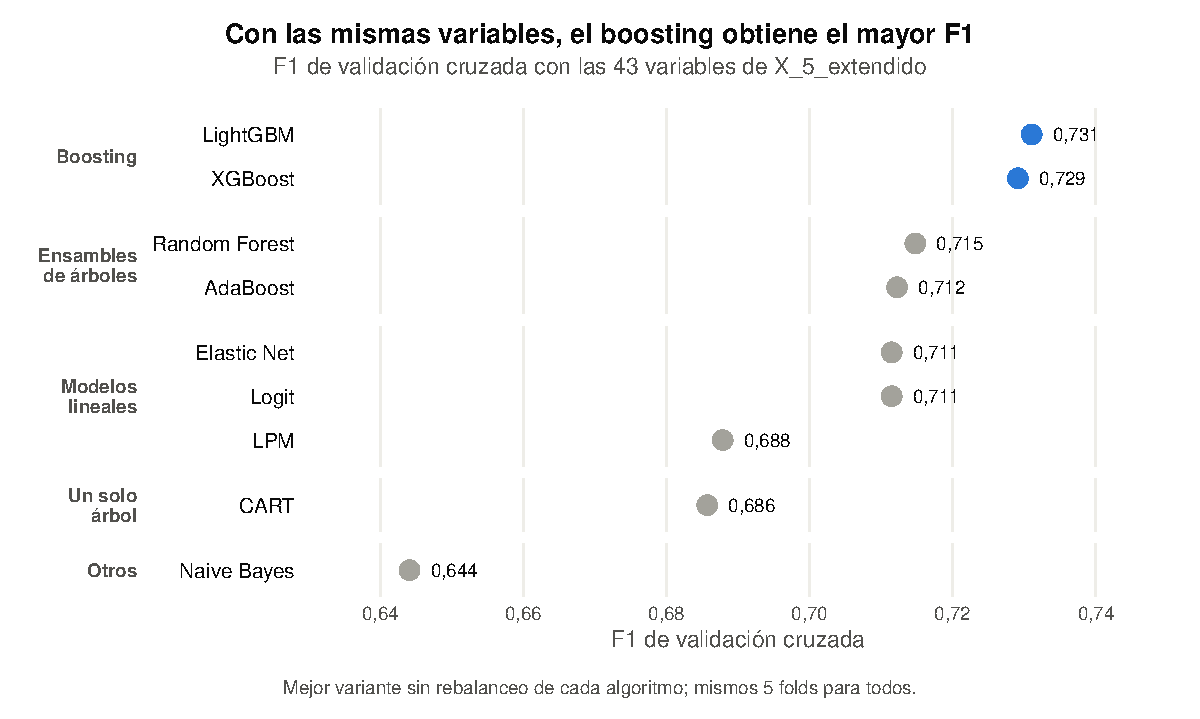
\includegraphics[width=\linewidth, height=0.82\textheight, keepaspectratio]{comparacion_algoritmos_x5}
    \end{column}
    \begin{column}{0.31\textwidth}
      \footnotesize
      \begin{itemize}
        \item El boosting (0,731 y 0,729) queda separado del resto.
        \item \textbf{Por qu\'e:} capta umbrales e interacciones sin que haya que especificarlas.
        \item Los ensambles y los modelos lineales quedan casi empatados (0,711 a 0,715).
        \item Un solo \'arbol (0,686) es inestable; Naive Bayes (0,644) supone variables independientes, y aqu\'i no lo son.
      \end{itemize}
    \end{column}
  \end{columns}
\end{frame}

\begin{frame}{A fondo: el boosting reduce el undercoverage}
  \centering
  {\small 
\begin{tabular}{lrrrrrr}
\toprule
Modelo & Umbral & Precisión & Recall & F1 & Falsos positivos & Falsos negativos\\
\midrule
LightGBM & 0,31 & 0,659 & 0,820 & 0,731 & 13.996 & 5.936\\
Random Forest & 0,34 & 0,651 & 0,792 & 0,715 & 13.985 & 6.880\\
Elastic Net & 0,35 & 0,670 & 0,758 & 0,711 & 12.316 & 7.989\\
\bottomrule
\end{tabular}
}

  \vspace{4mm}
  \begin{columns}[T, onlytextwidth]
    \begin{column}{0.48\textwidth}
      \footnotesize
      \begin{itemize}
        \item Falsos negativos = \textbf{undercoverage}: hogares pobres que quedar\'ian por fuera. Falsos positivos = \textbf{leakage}: hogares no pobres que recibir\'ian el beneficio.
        \item Frente a Elastic Net, LightGBM encuentra 2.053 hogares pobres m\'as, a cambio de 1.680 de leakage m\'as.
      \end{itemize}
    \end{column}
    \begin{column}{0.48\textwidth}
      \footnotesize
      \begin{itemize}
        \item Frente a Random Forest, encuentra 944 hogares pobres m\'as con el mismo leakage.
        \item Rivales: los dos algoritmos requeridos m\'as cercanos al boosting con X\_5 (Random Forest y Elastic Net), con los mismos folds.
      \end{itemize}
    \end{column}
  \end{columns}
  \nota{Validaci\'on cruzada en train (164.960 hogares). Cada modelo con el umbral que maximiza su F1.}
\end{frame}

\begin{frame}{A fondo: la ventaja no depende del umbral elegido}
  \begin{columns}[c, onlytextwidth]
    \begin{column}{0.64\textwidth}
      \centering
      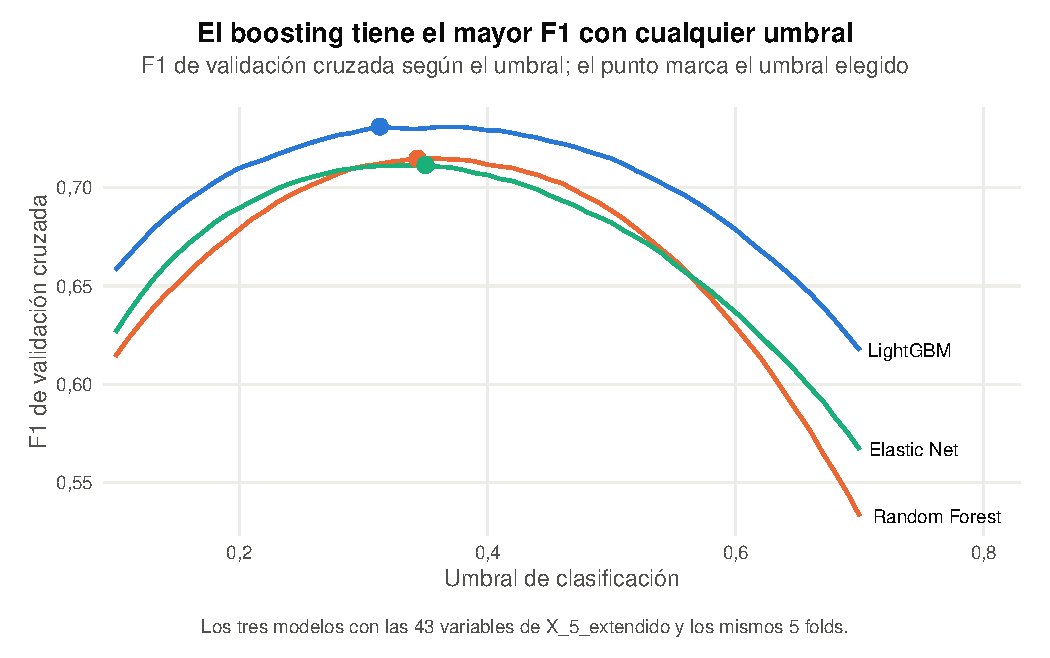
\includegraphics[width=\linewidth, height=0.82\textheight, keepaspectratio]{f1_umbral_top3}
    \end{column}
    \begin{column}{0.33\textwidth}
      \footnotesize
      \begin{itemize}
        \item LightGBM tiene el mayor F1 con cualquier umbral entre 0,10 y 0,70.
        \item Su ventaja no viene de haber escogido un buen umbral.
      \end{itemize}
    \end{column}
  \end{columns}
\end{frame}

\begin{frame}{A fondo: a igual cobertura, menos leakage}
  \begin{columns}[c, onlytextwidth]
    \begin{column}{0.64\textwidth}
      \centering
      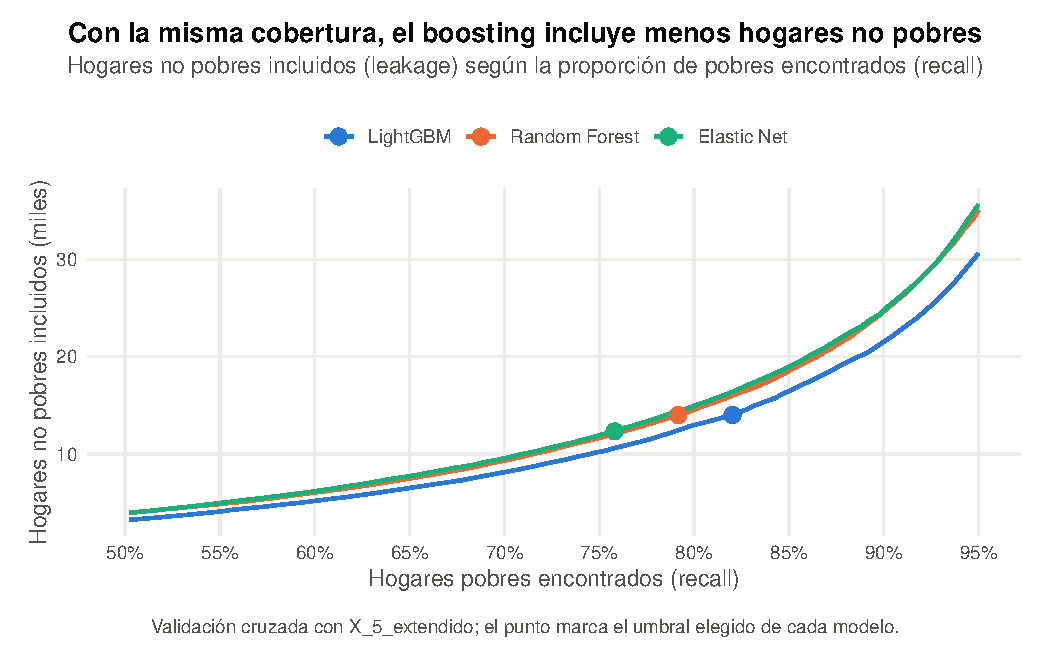
\includegraphics[width=\linewidth, height=0.82\textheight, keepaspectratio]{leakage_recall_top3}
    \end{column}
    \begin{column}{0.33\textwidth}
      \footnotesize
      \begin{itemize}
        \item Para encontrar al 80\% de los hogares pobres, LightGBM incluye 12.965 no pobres; Random Forest, 14.572; Elastic Net, 14.928.
        \item La curva de LightGBM queda por debajo en todo el rango: ordena mejor a los hogares de m\'as a menos probable de ser pobre.
        \item Por eso gana con cualquier balance entre leakage y undercoverage que prefiera la pol\'itica.
      \end{itemize}
    \end{column}
  \end{columns}
\end{frame}

\begin{frame}{A fondo: la misma informaci\'on, con otro peso}
  \centering
  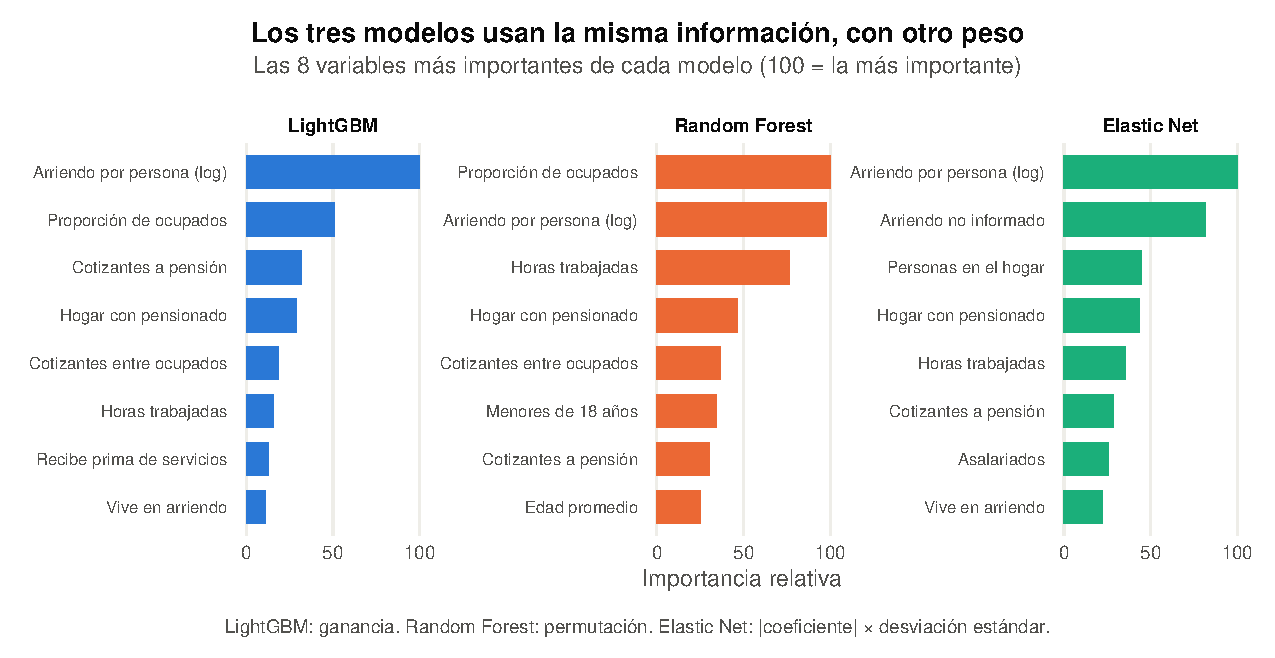
\includegraphics[width=\linewidth, height=0.62\textheight, keepaspectratio]{importancia_top3}

  \begin{columns}[T, onlytextwidth]
    \begin{column}{0.48\textwidth}
      \footnotesize
      \begin{itemize}
        \item Cuatro variables est\'an entre las 8 m\'as importantes de los tres modelos: arriendo por persona, hogar con pensionado, horas trabajadas y cotizantes a pensi\'on.
      \end{itemize}
    \end{column}
    \begin{column}{0.48\textwidth}
      \footnotesize
      \begin{itemize}
        \item La diferencia est\'a en c\'omo las usan: Elastic Net suma efectos lineales; los \'arboles las combinan con umbrales, y el boosting adem\'as corrige en cada ronda los errores de la anterior.
      \end{itemize}
    \end{column}
  \end{columns}
\end{frame}

% ============================================================
\section{Variables, ajuste y desbalance}
% ============================================================

\begin{frame}{M\'as informaci\'on sobre el hogar pesa m\'as que el algoritmo}
  \begin{columns}[c, onlytextwidth]
    \begin{column}{0.64\textwidth}
      \centering
      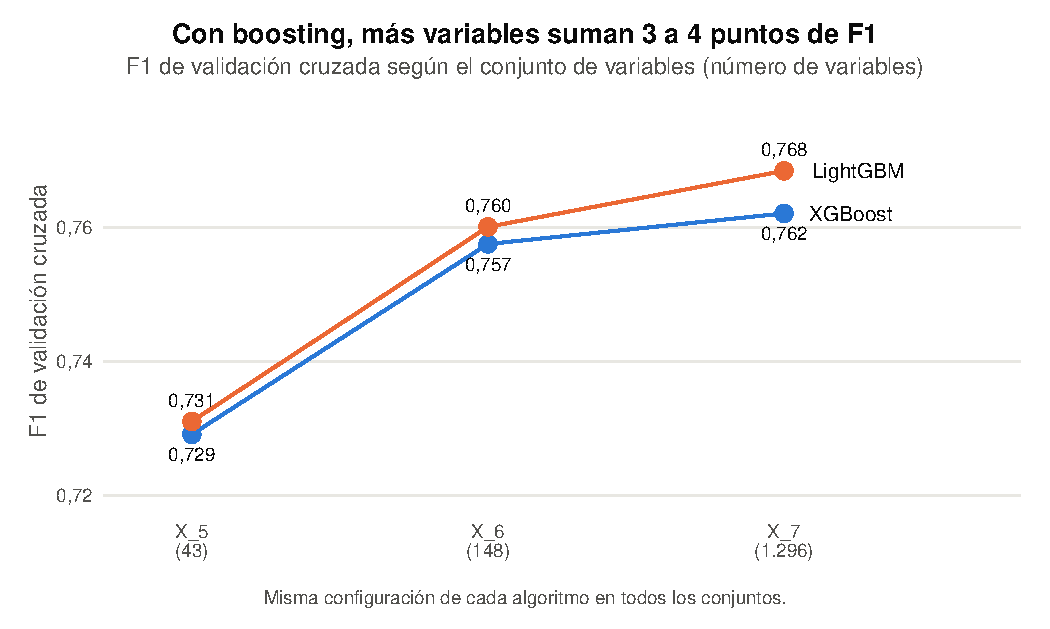
\includegraphics[width=\linewidth, height=0.82\textheight, keepaspectratio]{efecto_variables_boosting}
    \end{column}
    \begin{column}{0.33\textwidth}
      \footnotesize
      \begin{itemize}
        \item Con el mismo algoritmo, pasar de X\_5 a X\_6 (educaci\'on, ocupaci\'on y empresa de cada miembro) suma unos 3 puntos.
        \item X\_7 agrega menos de 1 punto m\'as con 1.148 variables adicionales: rendimientos decrecientes.
        \item Con X\_7, LightGBM supera a XGBoost por 0,6 puntos.
      \end{itemize}
    \end{column}
  \end{columns}
\end{frame}

\begin{frame}{Ajustar y rebalancear mueve poco el F1}
  \vspace{3mm}
  \begin{columns}[c, onlytextwidth]
    \begin{column}{0.66\textwidth}
      {\footnotesize\textbf{Ajuste de hiperpar\'ametros} (X\_5)\par\smallskip}
      \resizebox{\linewidth}{!}{
\begin{tabular}{lll}
\toprule
Variante & Hiperparámetros & F1 CV\\
\midrule
Elastic Net & alpha 0,25; lambda 0,0001 (elegidos por CV) & 0,711\\
Logit & Sin penalización & 0,711\\
Random Forest (fijo) & mtry 6, nodo mínimo 10, 300 árboles (fijos) & 0,704\\
Random Forest (grilla CV) & mtry 31, nodo mínimo 20, 300 árboles (elegidos por CV) & 0,715\\
\bottomrule
\end{tabular}
}
    \end{column}
    \begin{column}{0.31\textwidth}
      \footnotesize
      \begin{itemize}
        \item Elegir los hiperpar\'ametros de Random Forest por validaci\'on cruzada suma 1,1 puntos.
        \item Penalizar el logit (Elastic Net) no cambia el F1.
      \end{itemize}
    \end{column}
  \end{columns}
  \vspace{3mm}
  \begin{columns}[c, onlytextwidth]
    \begin{column}{0.66\textwidth}
      {\footnotesize\textbf{Rebalanceo de clases} (X\_5)\par\smallskip}
      \centering
      {\scriptsize 
\begin{tabular}{llll}
\toprule
Algoritmo & Rebalanceo & F1 CV & Umbral\\
\midrule
AdaBoost & Sin rebalanceo & 0,712 & 0,46\\
AdaBoost & Pobres x4 & 0,714 & 0,55\\
CART & Sin rebalanceo & 0,686 & 0,28\\
CART & Upsampling & 0,685 & 0,75\\
CART & Downsampling & 0,677 & 0,74\\
Naive Bayes & Sin rebalanceo & 0,644 & 0,88\\
Naive Bayes & Pobres x4 & 0,644 & 0,96\\
Random Forest (grilla CV) & Sin rebalanceo & 0,715 & 0,34\\
Random Forest (grilla CV) & Pobres x4 & 0,710 & 0,52\\
\bottomrule
\end{tabular}
}
    \end{column}
    \begin{column}{0.31\textwidth}
      \footnotesize
      \begin{itemize}
        \item Rebalancear cambia el F1 en menos de 1 punto, a veces para peor.
        \item Lo que cambia es el umbral: elegirlo para maximizar el F1 ya corrige el desbalance.
      \end{itemize}
    \end{column}
  \end{columns}
\end{frame}

% ============================================================
\section{Conclusi\'on}
% ============================================================

\begin{frame}{¿Qu\'e modelo le recomendar\'iamos al gobierno?}
  \vspace{5mm}
  \centering
  {\scriptsize
  \begin{tabular}{lrr>{\raggedright\arraybackslash}p{0.21\textwidth}>{\raggedright\arraybackslash}p{0.27\textwidth}}
    \toprule
    Modelo & F1 CV & Variables & ¿Se puede explicar? & Informaci\'on que exige \\
    \midrule
    LightGBM con X\_7 & 0,768 & 1.296 & Poco: cientos de \'arboles & Encuesta completa del hogar y de cada miembro \\
    LightGBM con X\_5 & 0,731 & 43 & Poco: cientos de \'arboles & Vivienda, composici\'on, empleo y arriendo \\
    Logit con X\_5 & 0,711 & 43 & S\'i: un coeficiente por variable & La misma de X\_5 \\
    CART con X\_5 & 0,686 & 43 & S\'i: reglas que se leen en un \'arbol & La misma de X\_5 \\
    \bottomrule
  \end{tabular}}

  \vspace{4mm}
  \begin{columns}[T, onlytextwidth]
    \begin{column}{0.48\textwidth}
      \footnotesize
      \begin{itemize}
        \item No necesariamente el de mayor puntaje: m\'as F1 exige m\'as informaci\'on y modelos m\'as dif\'iciles de explicar.
        \item Con las mismas 43 variables, pasar de un solo \'arbol al boosting suma 4,5 puntos; ampliar la informaci\'on a X\_7 suma 3,7 m\'as.
      \end{itemize}
    \end{column}
    \begin{column}{0.48\textwidth}
      \footnotesize
      \begin{itemize}
        \item El F1 pesa igual leakage y undercoverage. Si la agencia prefiere no dejar pobres por fuera, basta bajar el umbral, sin cambiar de modelo.
        \item \textbf{Propuesta:} boosting con un conjunto corto de variables f\'aciles de verificar, y un modelo explicable como referencia para justificar a qui\'en se focaliza.
      \end{itemize}
    \end{column}
  \end{columns}
\end{frame}

% ============================================================
\appendix

\begin{frame}[standout]
  ¡Gracias!
\end{frame}

\end{document}